\documentclass[conference]{IEEEtran}
\IEEEoverridecommandlockouts
% The preceding line is only needed to identify funding in the first footnote. If that is unneeded, please comment it out.
\usepackage{cite}
\usepackage{amsmath,amssymb,amsfonts}
\usepackage{algorithmic}
\usepackage{graphicx}
\usepackage{multicol}
\usepackage{minted}
\usepackage{textcomp}
\usepackage{xcolor}

\def\BibTeX{{\rm B\kern-.05em{\sc i\kern-.025em b}\kern-.08em
    T\kern-.1667em\lower.7ex\hbox{E}\kern-.125emX}}
\begin{document}
\title{Paper Reading of \textit{Coverage-Guided Tensor Compiler Fuzzing with JointIR-Pass Mutation}}

\author{\IEEEauthorblockN{Yiwei Yang}
    \IEEEauthorblockA{\textit{School of Information Science and Technology} \\
        \textit{ShanghaiTech University}\\
        Shanghai, China \\
        yangyw@shanghaitech.edu.cn}
}

\maketitle

\begin{abstract}
    The Machine Learning System is surging these days providing good compiler and system infrastructure for Machine Learning training. When developing the DK System, bugs could occur ant application level, library level and infrastructure level. The paper think the bugs in DL library like TVM are significant for the application. Compared with latest Libfuzzer, TVMFUzz(A Type-Directed Relay Fuzzing Library) \cite{b3} and LEMON \cite{b2}, the paper introduced a new fuzzing tool on TVM RelayTIRs to auto-generate ops and coverage guided auto-generation, which have better performance than LEMON, LibFuzzer and TVMFuzz. For future fuzzing for Tensor Compiler like TVM or MLIR, we actually can build shape inference based generator to better construct meaningful and usable shape to fuzz the compiler, that may fuzz more parts in the compiler not just the backend.

    \begin{figure}[htbp]
        \centering
        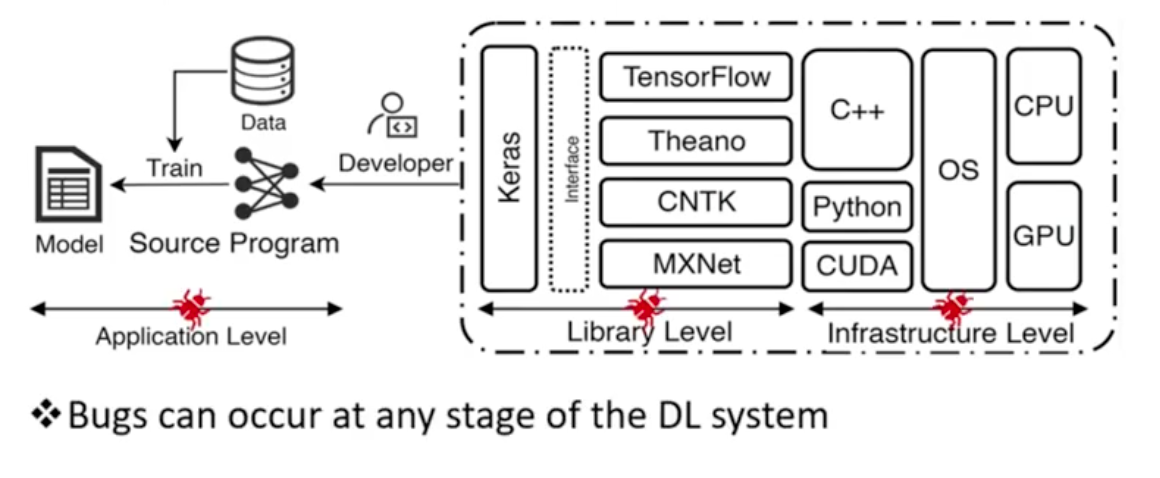
\includegraphics[width=\columnwidth]{./lemon.png}
        \caption{}
    \end{figure}
\end{abstract}

\begin{IEEEkeywords}
    MLSys, fuzzing, coverage guided
\end{IEEEkeywords}

\section{Paper Summary}
Tzer is a Fuzzing framework based on TVM Relay IR and TVM IR. Mutators are defined over operators of Relay and TVM IR to generate IR struct to better detect the bugs in TVM.
\begin{figure}[htbp]
    \centering
    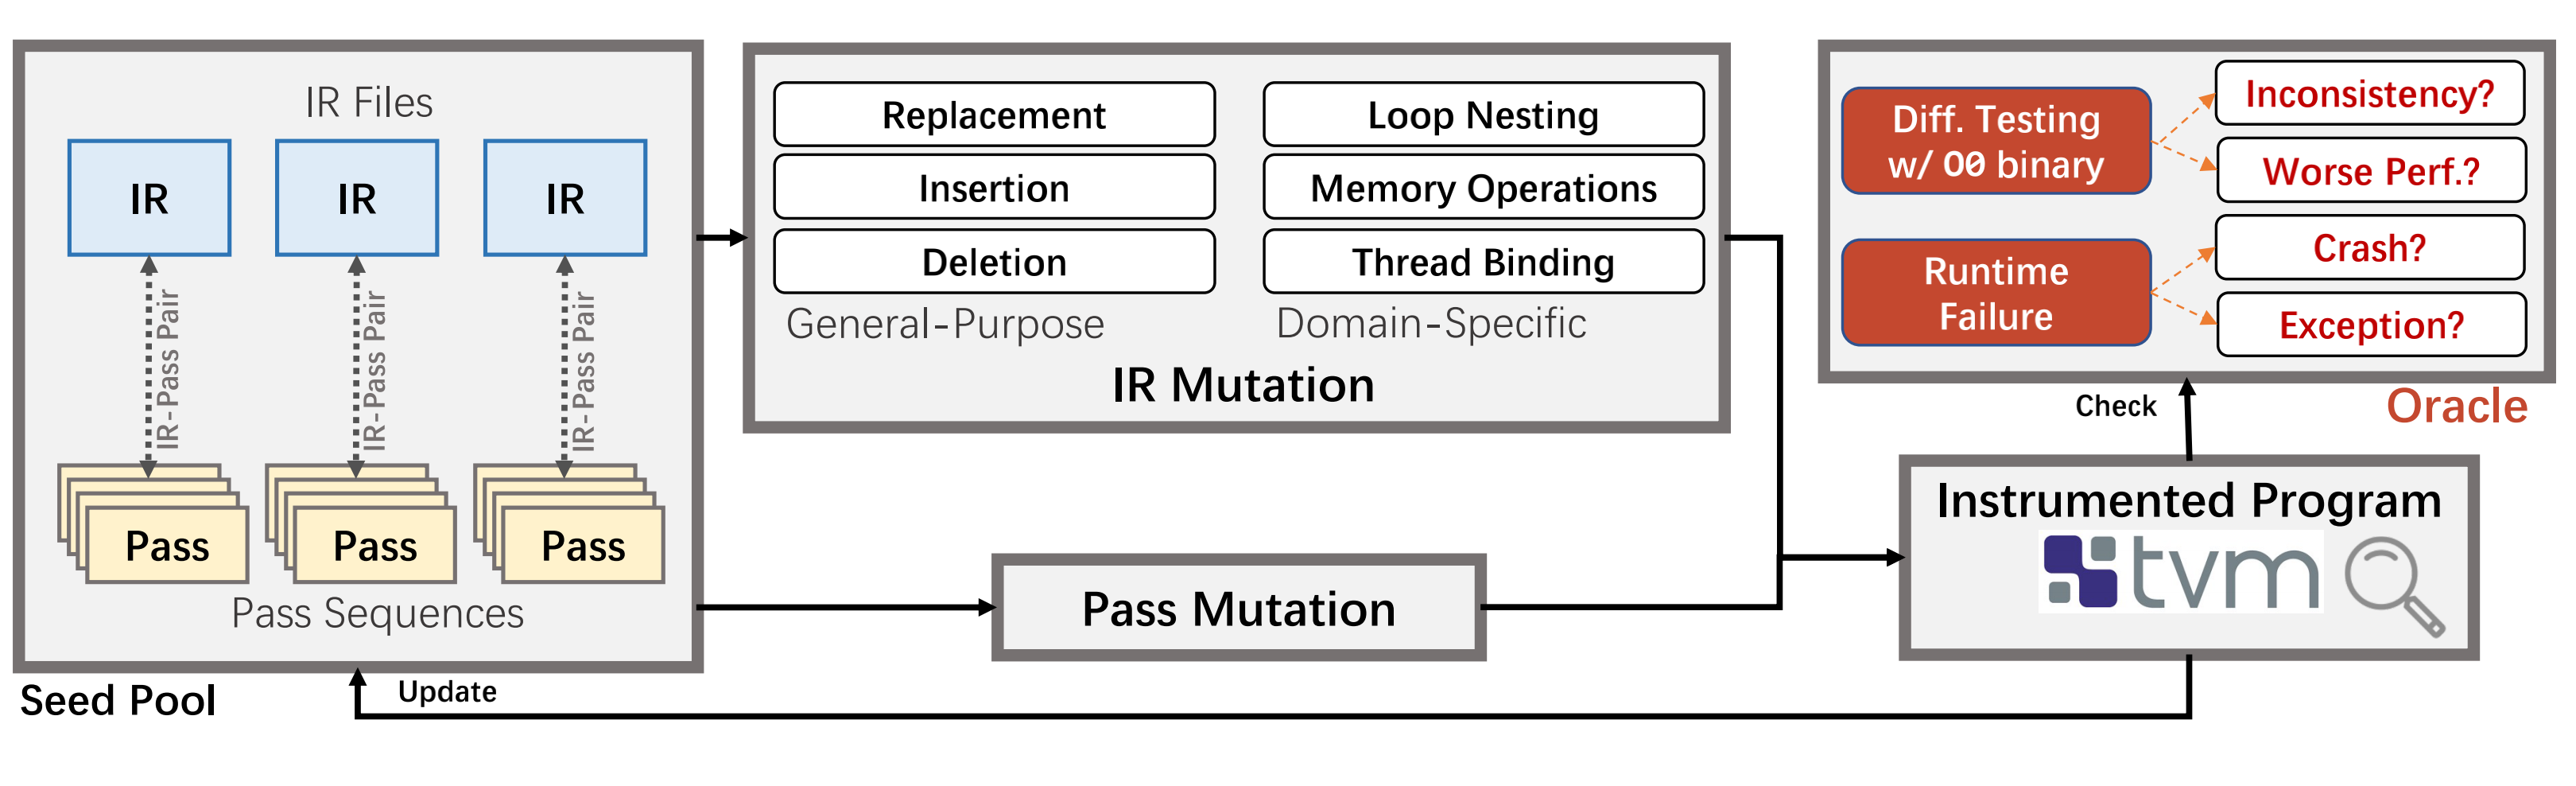
\includegraphics[width=\columnwidth]{./tzer_overview.png}
    \caption{Overview of Tzer}
  \end{figure}
There exists General Purpose fuzzing and Domain-Specific Mutation on the IR.
General Purpose fuzzing is to assure syntax correctness and prevent semantic problems, mutation incorporates program analysis techniques.

\begin{figure}[htbp]
    \centering
    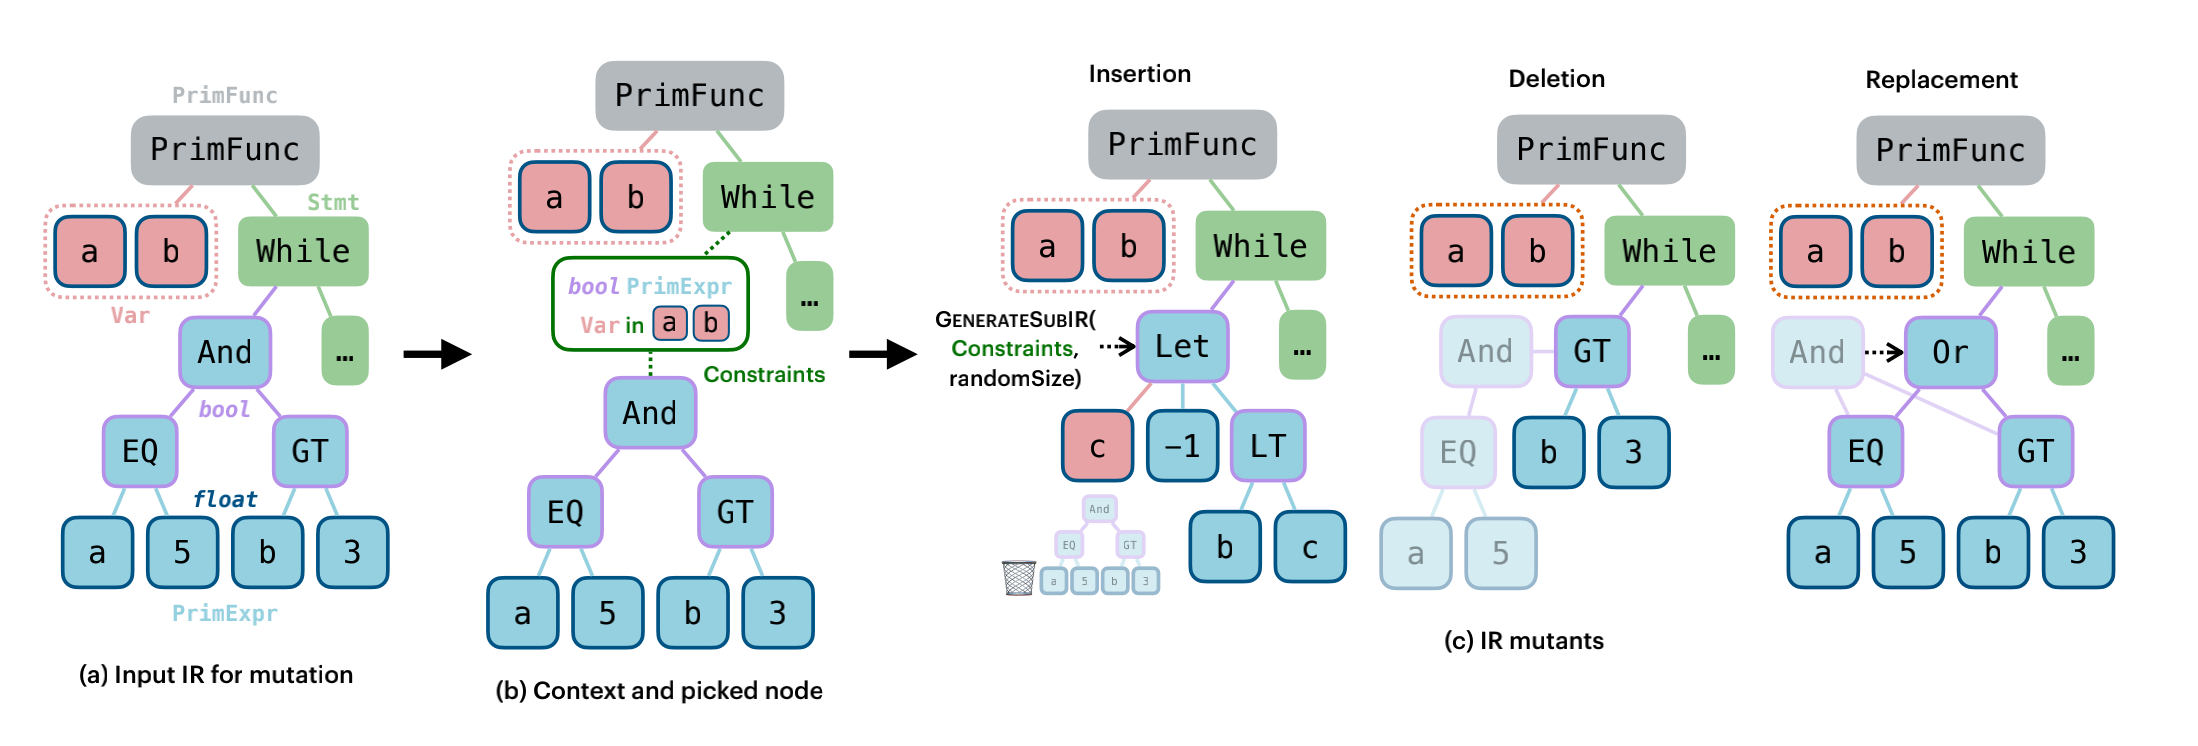
\includegraphics[width=\columnwidth]{./mutation_process.png}
    \caption{IR Mutation Process of Tzer}
  \end{figure}
  The result of coverage is obviously better than LEMON and TVMFuzz. Using LEMON seeds makes valuable tests more fruitful. The sensitivity to Pass Mutation frequency and fuzzing time reduces quickly. Tzer found bugs like  Invalid Memory Access,  Python-C++ FFI Handling, API Misuse, API Inconsistency,  Type Error, Driver Lifetime Error, Out-of-Memory, Arithmetic Error and other bugs.
\section{Positive}
Tzer is obviously a more effective fuzzer than other counterpart.
\begin{figure}[htbp]
    \centering
    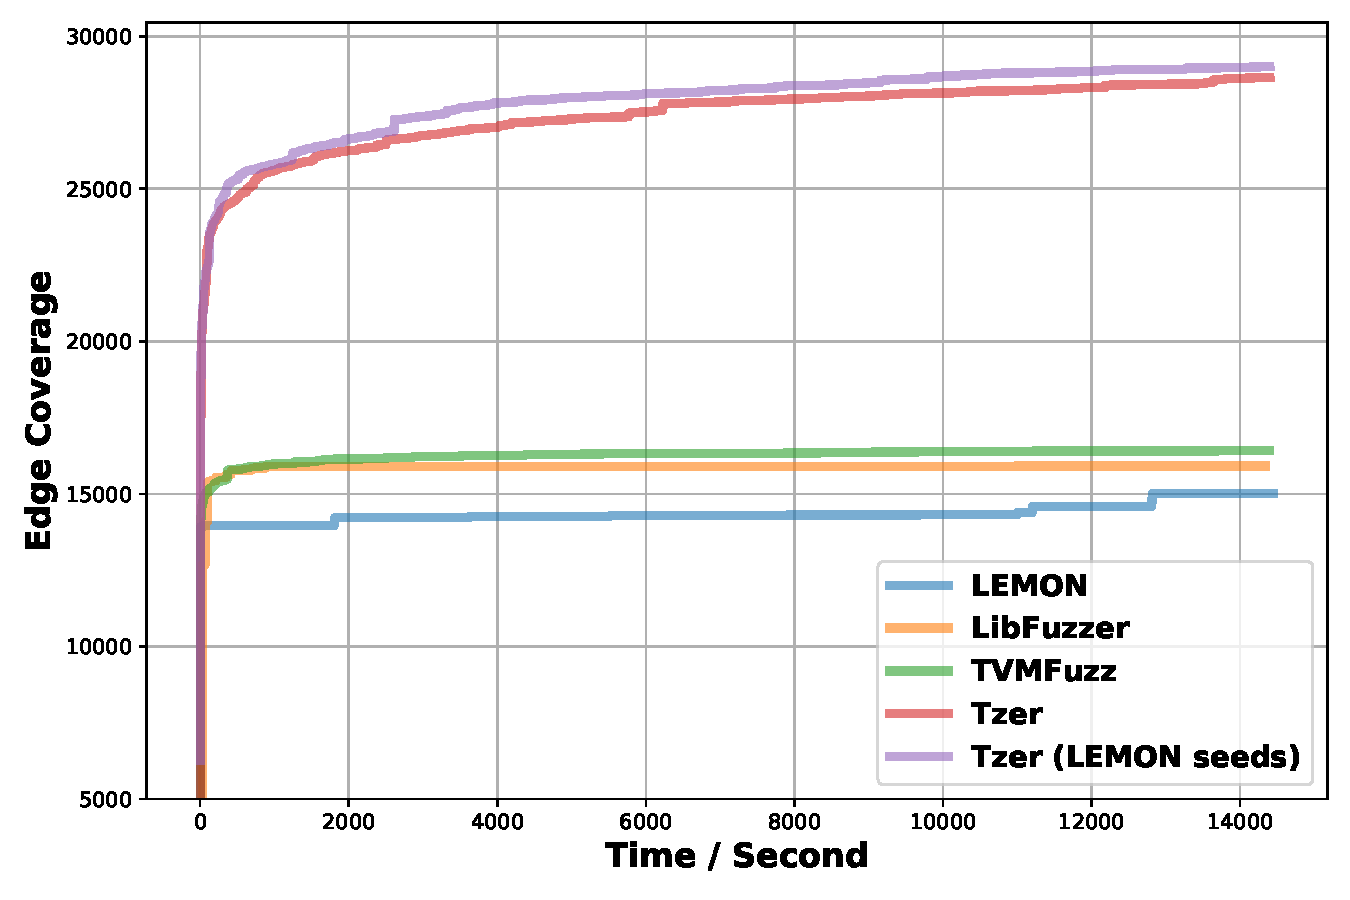
\includegraphics[width=\columnwidth]{./baseline_cov.pdf}
    \caption{Compared with Baseline}
  \end{figure}
  
\section{Negative}
The implementation is still based on the traditional mutator on IR, which is coverage guided Tensor generation. The author just migrate a relatively good work into the new area, not that fancy or focusing more on the essence of relay generation. Semantic bugs are still the main bugs they found.

\section{Soundness}
The following metrics are applied to evaluate the performance of Tzer and the compared techniques:
\subsection{Code Coverage} It's a normal metric to evaluate the coverage of the fuzzing tools. The coverage is defined as the number of IR nodes that are covered by the fuzzing tools. But personally, the better coverage of a tool is just to say it could reach the all paths of one program, not necessarily meaning it's ability to find bugs.
\subsection{The total number of useful tests} Following previous fuzzing work,  the number of created valuable tests, i.e., tests that are not only valid (i.e., compilable) but also contribute new coverage during the fuzzing process, for each comparison technique. The amount of syntactically/semantically valid tests with new coverage might largely reflect the number of novel system behaviors/paths covered/tested, hence this measure is critical. Also, because strategies that predominantly create incorrect inputs can nonetheless obtain high coverage for the error-handling code, this metric can be used to supplement code coverage, which is clearly not what we want.
\subsection{Number of Detected Bugs}  The number of previously unknown bugs detected by all of the analyzed strategies are also reported, since bug identification is the ultimate goal for such techniques. We classify distinct bugs in this paper based on how they are essentially fixed.
\section{Significance}
In terms of bugs found, the significance of the bugs and the number of bugs are nearly ten times of the previous work.

\section{Novelty}
The Domain-Specific part is the main novelty of this project. Domain-Specific specializes in programming containing a lot of loops. Existing tensor compilers use the idea of pass to optimize the supplied IR or include annotations holding vital information for subsequent optimization to optimize certain hot spot program structures. General-purpose mutators, while adaptable in handling multiple sorts of expressions, are nevertheless inefficient and not specialized to the specific domain that tensor compilers are created for when it comes to triggering the complicated logic underlying those optimization runs.
\subsection{Loop Nesting}

\section{Verifiability}


\section{Connection}

\section{Brainstorming}
I think the fuzzing over the IR is language level and the generated IR does not make production level sense. A more generic ONNX model fuzzer like CSmith should be created.
\subsection{ONNSMITH: A Neral Network Model Generation based on elemnt-wise}
The middle end of TVM or MLIR already has shape inference given the neural network and some data feed. We could leverage this information and cast mutation on that. The effectiveness of LEMON is imporior mainly because it relies on Hand written Neuron Effect Block mutation rule and the Metrics are not the assurance of correctness, just to maintain the generation of the model is correct. Plus, it only support the element wise operation.
Thus, ONNSMITH that utilize the symbolic shape inference function and restriction on symbolic, the fuzzer will. leverage the real model inference.
\begin{figure}[htbp]
    \centering
    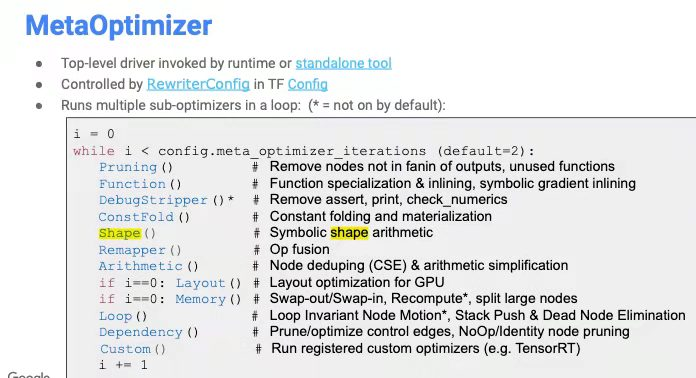
\includegraphics[width=\columnwidth]{./WechatIMG15.jpeg}
    \caption{Symbolic Shape Analysis for Optimizer}
  \end{figure}
  \subsection{RL Fuzzer for MLSys}
As a bachelor of fuzzer, I think the coverage graph is similar to Deep RL, that use seed(hyper parameter) to optimize the Q function(Mutator propagation) and to reach all the state in Neural Network(all triggered bugs) to make them response to remember the previous appeared state(fix bugs).

RL Fuzzer have been widely used in Fuzzer currently, but not yet in MLSys, but since x for MLSys is hot, RL for fuzzer should be hot, too. The Fuzzer will gain more information other than system bugs like semantic or Computer Arch but real neural network semantic bugs.
  
\begin{thebibliography}{00}
    \bibitem{b1} LIU, Jiawei, et al. Coverage-Guided Tensor Compiler Fuzzing with Joint IR-Pass Mutation. arXiv preprint arXiv:2202.09947, 2022.
    \bibitem{b2} WANG, Zan, et al. Deep learning library testing via effective model generation. In: Proceedings of the 28th ACM Joint Meeting on European Software Engineering Conference and Symposium on the Foundations of Software Engineering. 2020. p. 788-799.
    \bibitem{b3} SHEN, Qingchao, et al. A comprehensive study of deep learning compiler bugs. In: Proceedings of the 29th ACM Joint Meeting on European Software Engineering Conference and Symposium on the Foundations of Software Engineering. 2021. p. 968-980.
\end{thebibliography}
\end{document}
